\documentclass[aspectratio=169]{beamer}
\usepackage[framemethod=tikz]{mdframed}
\usepackage{pgfplots}
\usepackage{tikz}
\usepackage{url}
\usepackage{xcolor}
\usepackage{qrcode}
\usepackage{xmpmulti}
\usetikzlibrary{shapes,arrows}
\hypersetup{pdfstartview={Fit}} % Fit the presentation to the window when first displayed
\usetheme{Singapore}
\usecolortheme{orchid}
\pgfplotsset{compat=1.14}
\beamertemplatenavigationsymbolsempty{} % Remove Beamer navigation symbols
\nonstopmode{} % Keep making the file through errors
\usepackage[sfdefault]{sourcesanspro}
\usepackage[T1]{fontenc}

% Adapted from:
% http://danielfalster.com/blog/2013/06/18/a-nice-title-page-for-beamer-presentations/
\newmdenv[tikzsetting={draw=black,fill=white,fill opacity=0.85, line width=1pt},backgroundcolor=none,leftmargin=0,rightmargin=0,innertopmargin=5pt,skipbelow=\baselineskip,skipabove=\baselineskip]{TitleBox}

\title{Getting Started with Meshtastic}
\author[Swartz]{Tom~Swartz}
\institute{Central PA Open Source Conference}
\date{April 6 2024}
\subject{Computer Science}
\begin{document}


%- Introduction
%  - Brief explanation on current state of various LoRa protocols
%  - Overview of Meshtastic devices/software
%- Meshtastic Software in Detail
%  - Architecture and Design of Home Assistant
%  - Overview of sub-protocols, long range modes vs short range modes
%  - Network Security/Encryption vs Amateur Radio modes
%- Meshtastic Hardware in Detail
%  - Various Open Source Hardware examples
%- Making Custom Meshtastic Sensors
%  - Custom Temperature Sensors
%  - Integration with existing Internet-of-Things devices and Services

% Title Page
{\usebackgroundtemplate{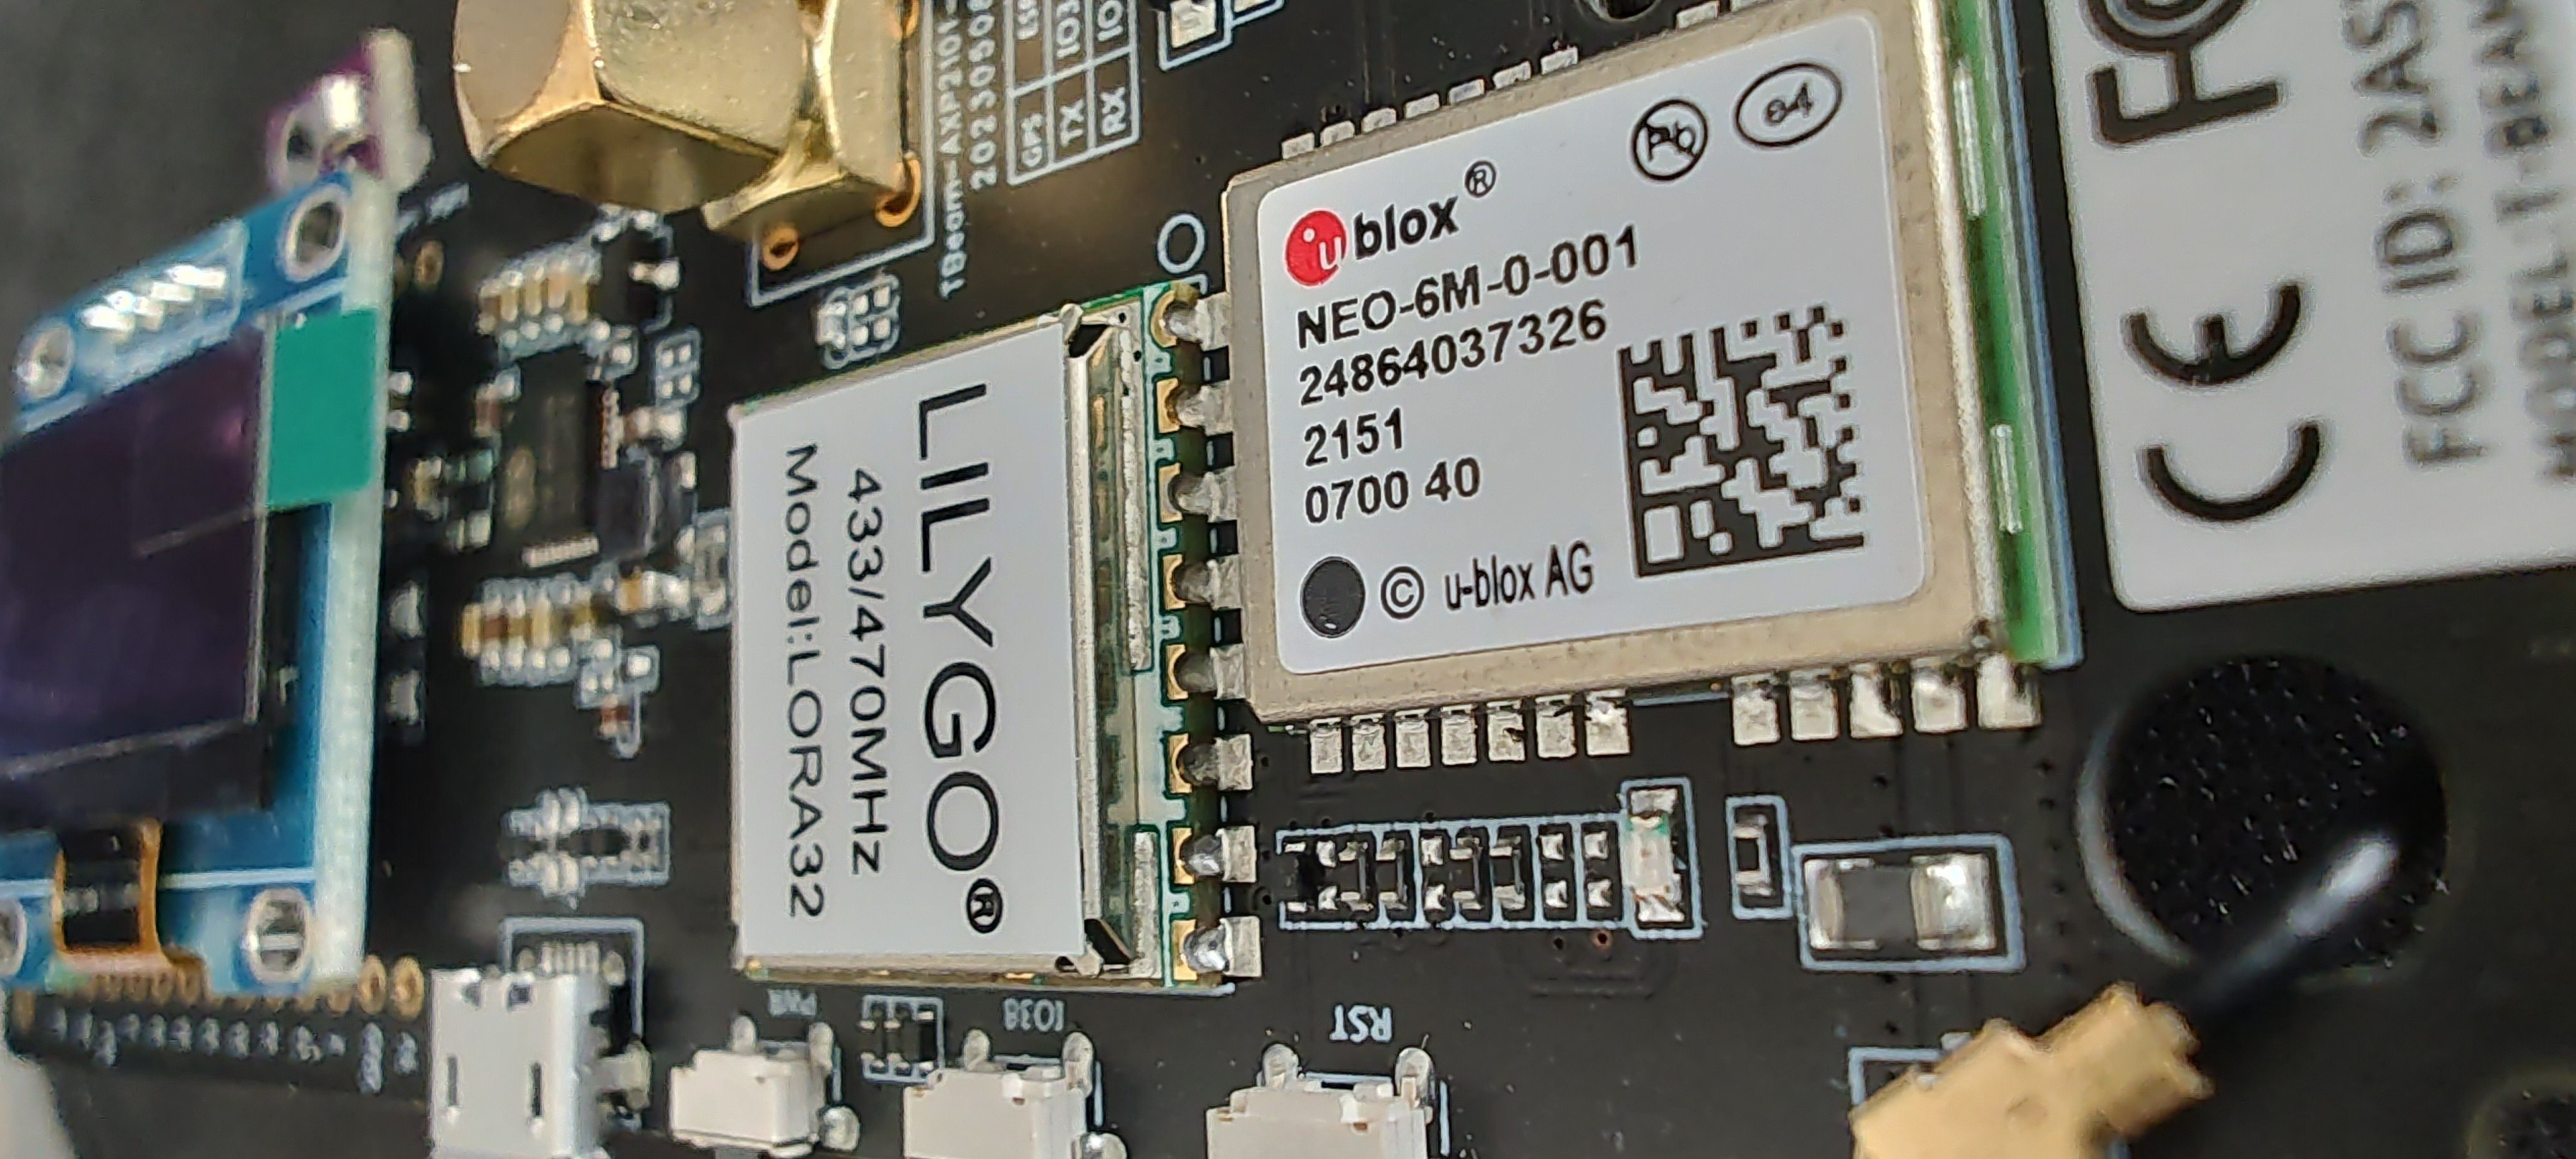
\includegraphics[width=1.00\paperwidth,height=1.0\paperheight]{images/tbeam-board.jpg}}
\begin{frame}[plain]
    \begin{TitleBox}
        \begin{center}
            {\color{red}\Large\inserttitle\color{black}}\\
        \end{center}
        \insertauthor{}\hfill\textbf{\insertinstitute{}}\hfill\insertdate{}\\
        {\footnotesize
        \href{https://hachyderm.io/@tswartz07}{@tswartz07@hachyderm.io}
        \hfill{}
        \href{mailto: tom@tswartz.net}{tom@tswartz.net}
        }
    \end{TitleBox}
    \vspace{15em}
\end{frame}}

\begin{frame}
  \frametitle{Who is this guy?}
  \framesubtitle{And what is he doing here?}
  \begin{columns}[]
    \begin{column}[T]{0.45\paperwidth}
      {\huge{Tom Swartz}}
      \vfill{}
      \begin{itemize}[<+->]
        \item{Crunchy Data \\ Associate Director of Support}
        \item{Hobbyist interests in `Big Data', IoT, RF Communications}
        \item{Prior CPOSC talks on RF comms/SDR \& homemade PCBs}
        \item{I've got some pretty specific hyperfixations}
      \end{itemize}
    \end{column}
    \begin{column}[T]{0.45\paperwidth}
      
\includegraphics[height=6cm,keepaspectratio]{images/logo.png}
    \end{column}
  \end{columns}
\end{frame}

\section{What's all this then?}
\begin{frame}
  \frametitle{Summary}
  We'll be reviewing the following topics, and how they relate to Meshtastic
  \begin{enumerate}
    \item{The LoRa Ecosystem}
    \item{Meshtastic Software and Hardware in Detail}
    \item{Building Your Own Mesh Network with Custom Sensors}
  \end{enumerate}
\end{frame}

\subsection{The LoRa Ecosystem}
\frame{\subsectionpage}

\begin{frame}[fragile]
  \frametitle{What is LoRa?}
  \begin{columns}[]
    \begin{column}[T]{0.45\paperwidth}
      \begin{itemize}%[<+->]
        \item{There are a variety of \color{red}{Lo}\color{black}ng \color{red}{Ra}\color{black}nge (LoRa) wireless communication protocols}
        \item{Most are based on Semtech patented methods}
        \item{Nearly all use license-free (no ham radio) RF bands}
        \item{Can easily attain 6+ mile range}
     \end{itemize}
    \end{column}
    \begin{column}[T]{0.45\paperwidth}
      %
\includegraphics[height=4cm,keepaspectratio]{images/standards.png}
    \end{column}
  \end{columns}
\end{frame}

\begin{frame}[fragile]
  \frametitle{So, what is Meshtastic then?}
  \begin{columns}[]
    \begin{column}[T]{0.45\paperwidth}
      \begin{itemize}%[<+->]
        \item{Yet one more standard!}
        \item{Meshtastic uses LoRa P2P with a custom, Open Source protocol aimed at consistent, long distance text communication}
        \item{The actual protocol is Open Source!}
        \item{Focus on using license-free RF bands, with allowances for Amateur Radio modes}
        \item{Currently holds record for longest distance of the LoRa family- 254KM (158 miles)!}
     \end{itemize}
    \end{column}
    \begin{column}[T]{0.45\paperwidth}
      
\includegraphics[height=4cm,keepaspectratio]{images/standards.png}
    \end{column}
  \end{columns}
\end{frame}

\begin{frame}[fragile]
  \frametitle{``But, I have a Cell Phone?''}
  \begin{columns}[]
    \begin{column}[T]{0.45\paperwidth}
      Reasons for using Meshtastic aren't to `replace' existing infrastructure, but to supplement it.
      \begin{itemize}%[<+->]
        \item{Things happen!}
        \item{Meshtastic doesn't depend on wider infrastructure}
        \item{Meshtastic can be completely privately encrypted, in certain situations}
        \item{Platform for experimentation}
        \item{No ongoing `fees' associated with usage}
     \end{itemize}
    \end{column}
    \begin{column}[T]{0.45\paperwidth}
      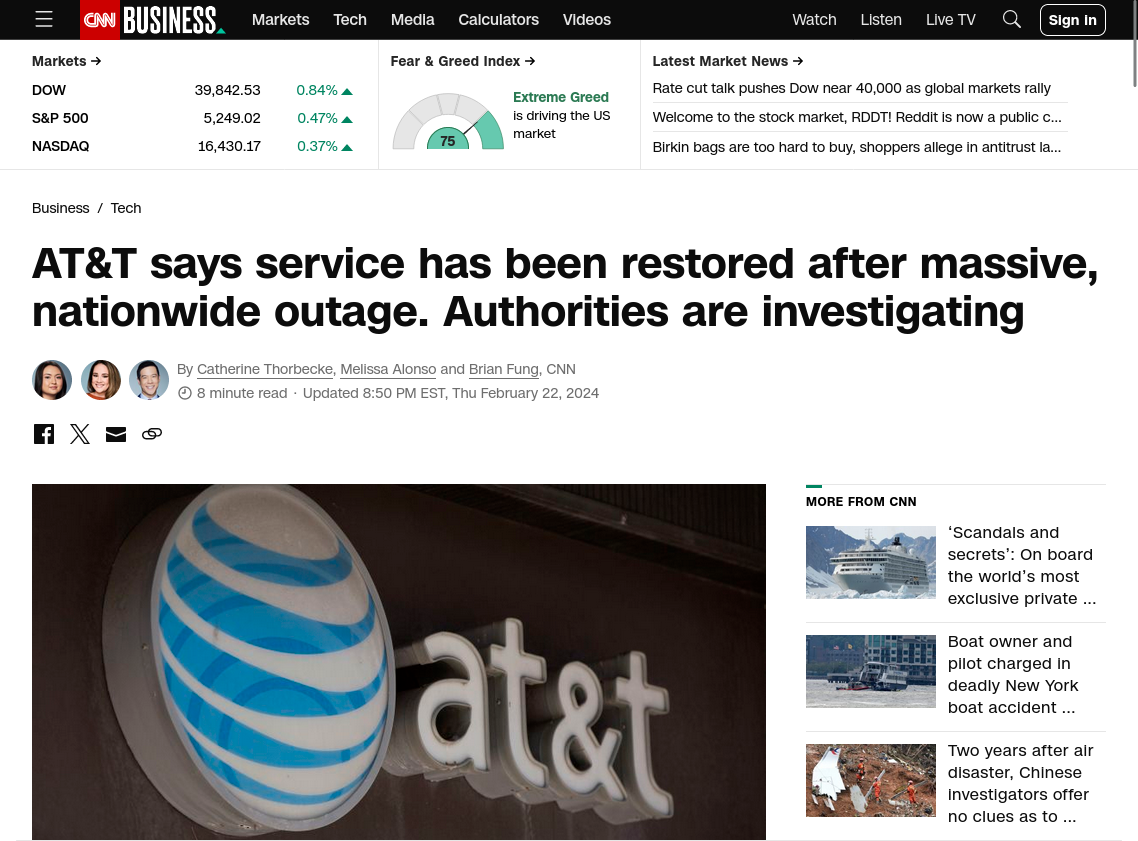
\includegraphics[height=5cm,keepaspectratio]{images/att.png}
    \end{column}
  \end{columns}
\end{frame}

%\begin{frame}[fragile]
%  \frametitle{How does Meshtastic compare?}
%  \begin{columns}[]
%    \begin{column}[T]{0.45\paperwidth}
%      \Large{General LoRa (LoRaWAN, GoTenna Mesh)}
%      \begin{itemize}
%        \item{Sometimes proprietary}
%        \item{Semi-strict definitions for messaging and position}
%        \item{GoTenna went corpo}
%      \end{itemize}
%    \end{column}
%    \begin{column}[T]{0.45\paperwidth}
%      \Large{Meshtastic}
%      \begin{itemize}
%        \item{Based on an open hardware spec}
%        \item{Support for a variety of external modules}
%        \item{Currently holds the longest range of all LoRa varieties}
%      \end{itemize}
%    \end{column}
%  \end{columns}
%\end{frame}

% Install Methods
\begin{frame}[fragile]
  \frametitle{Getting Started}
  \begin{columns}[]
    \begin{column}[T]{0.35\paperwidth}
      \begin{enumerate}%[<+->]
        \item{Buy/Build hardware}
        \item{Flash Firmware}
        \item{Power it on, pick Region}
        \item{There is no Step 4!}
      \end{enumerate}
    \end{column}
    \begin{column}[T]{0.55\paperwidth}
      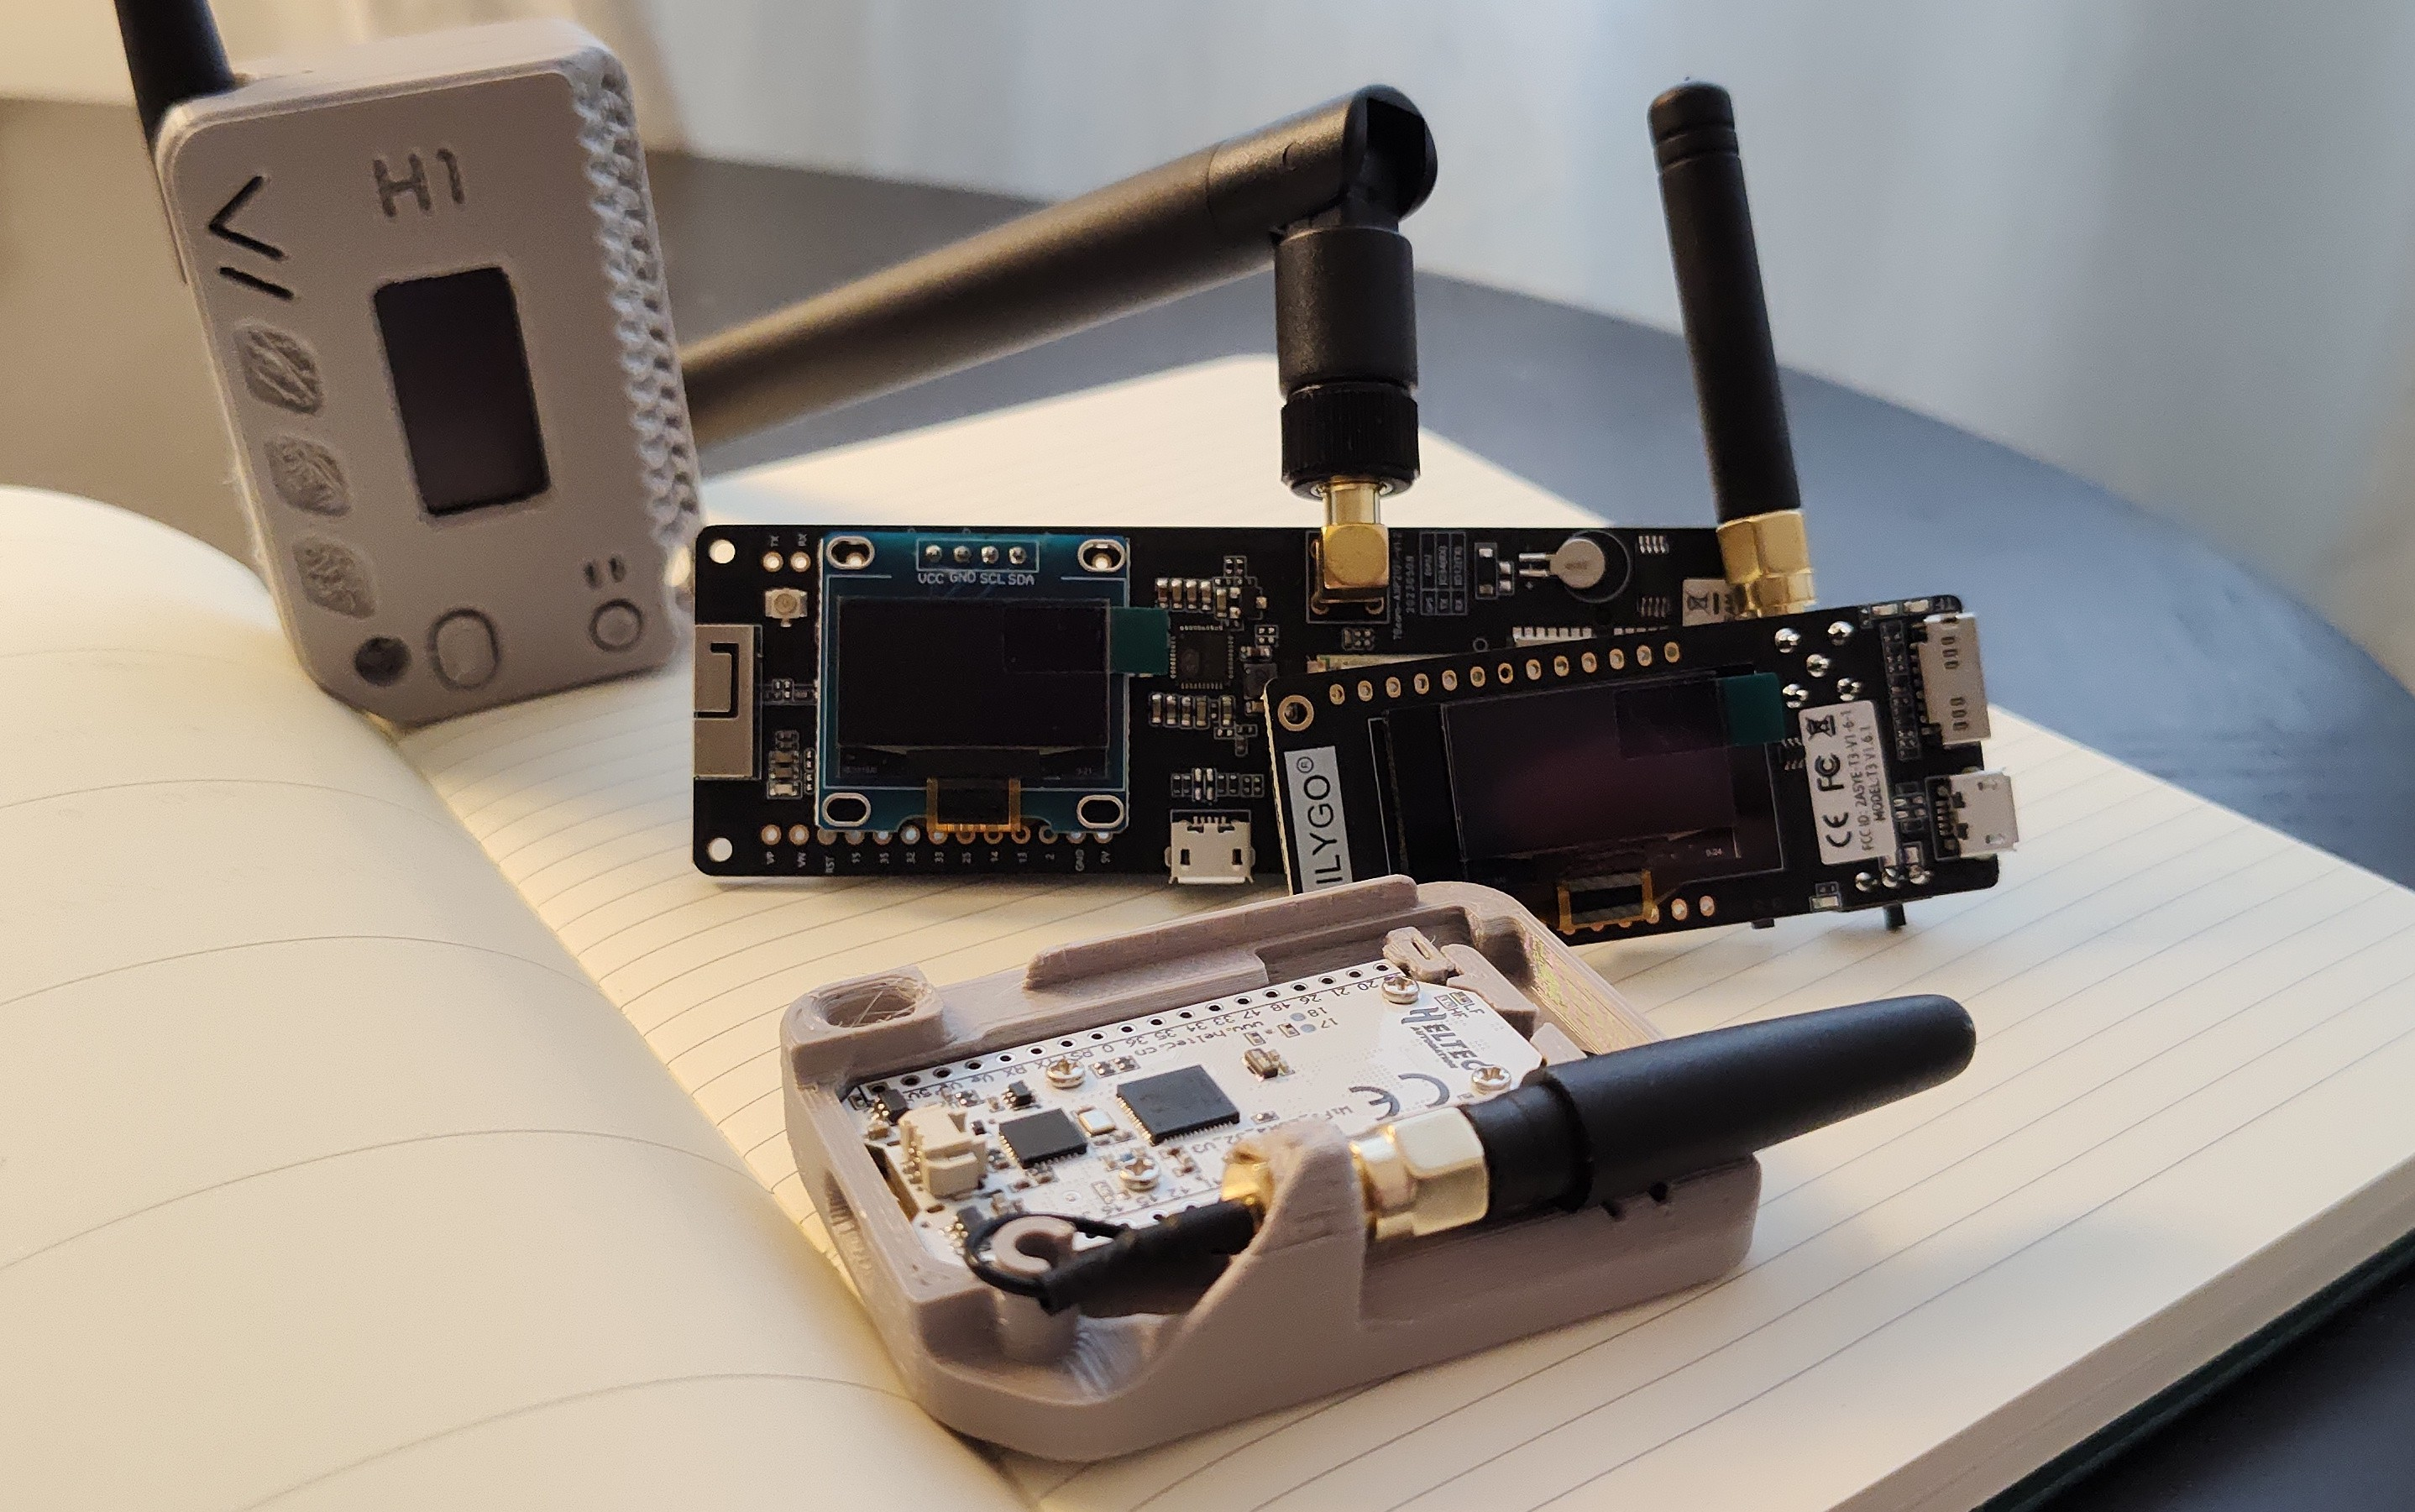
\includegraphics[height=5.5cm,keepaspectratio]{images/boards.jpg}
    \end{column}
  \end{columns}
\end{frame}

\section{Meshtastic In Detail}
\subsection{Meshtastic Hardware in Detail}
\begin{frame}[fragile]
  \frametitle{Meshtastic Hardware in Detail}
  There are a wide variety of devices, but they fall into three categories:
  \begin{description}%[<+->]
    \item[ESP32]{Older, power-hungry, but common. Supports Bluetooth and WiFi}
    \item[nRF52]{Newer, \emph{significantly} lower power, easier to manage, lacks WiFi}
    \item[RP2040]{Newest, ARM-based, can do wired Ethernet}
  \end{description}
  \vfill{}
  \emph{Worth noting that some devices lack certain features (such as GPS, screens, etc.)}
\end{frame}

\subsection{Meshtastic Software in Detail}
\begin{frame}[fragile]
  \frametitle{Meshtastic Software in Detail}
  \vfill{}
  \begin{columns}[]
    \begin{column}[T]{0.45\paperwidth}
      \begin{enumerate}%[<+->]
        \item{Peer to Peer protocol}
        \item{Uses custom Chirp Spread Spectrum}
        \item{Variety of `Modem Presets' for differing environments}
      \end{enumerate}
    \end{column}
    \begin{column}[T]{0.45\paperwidth}
      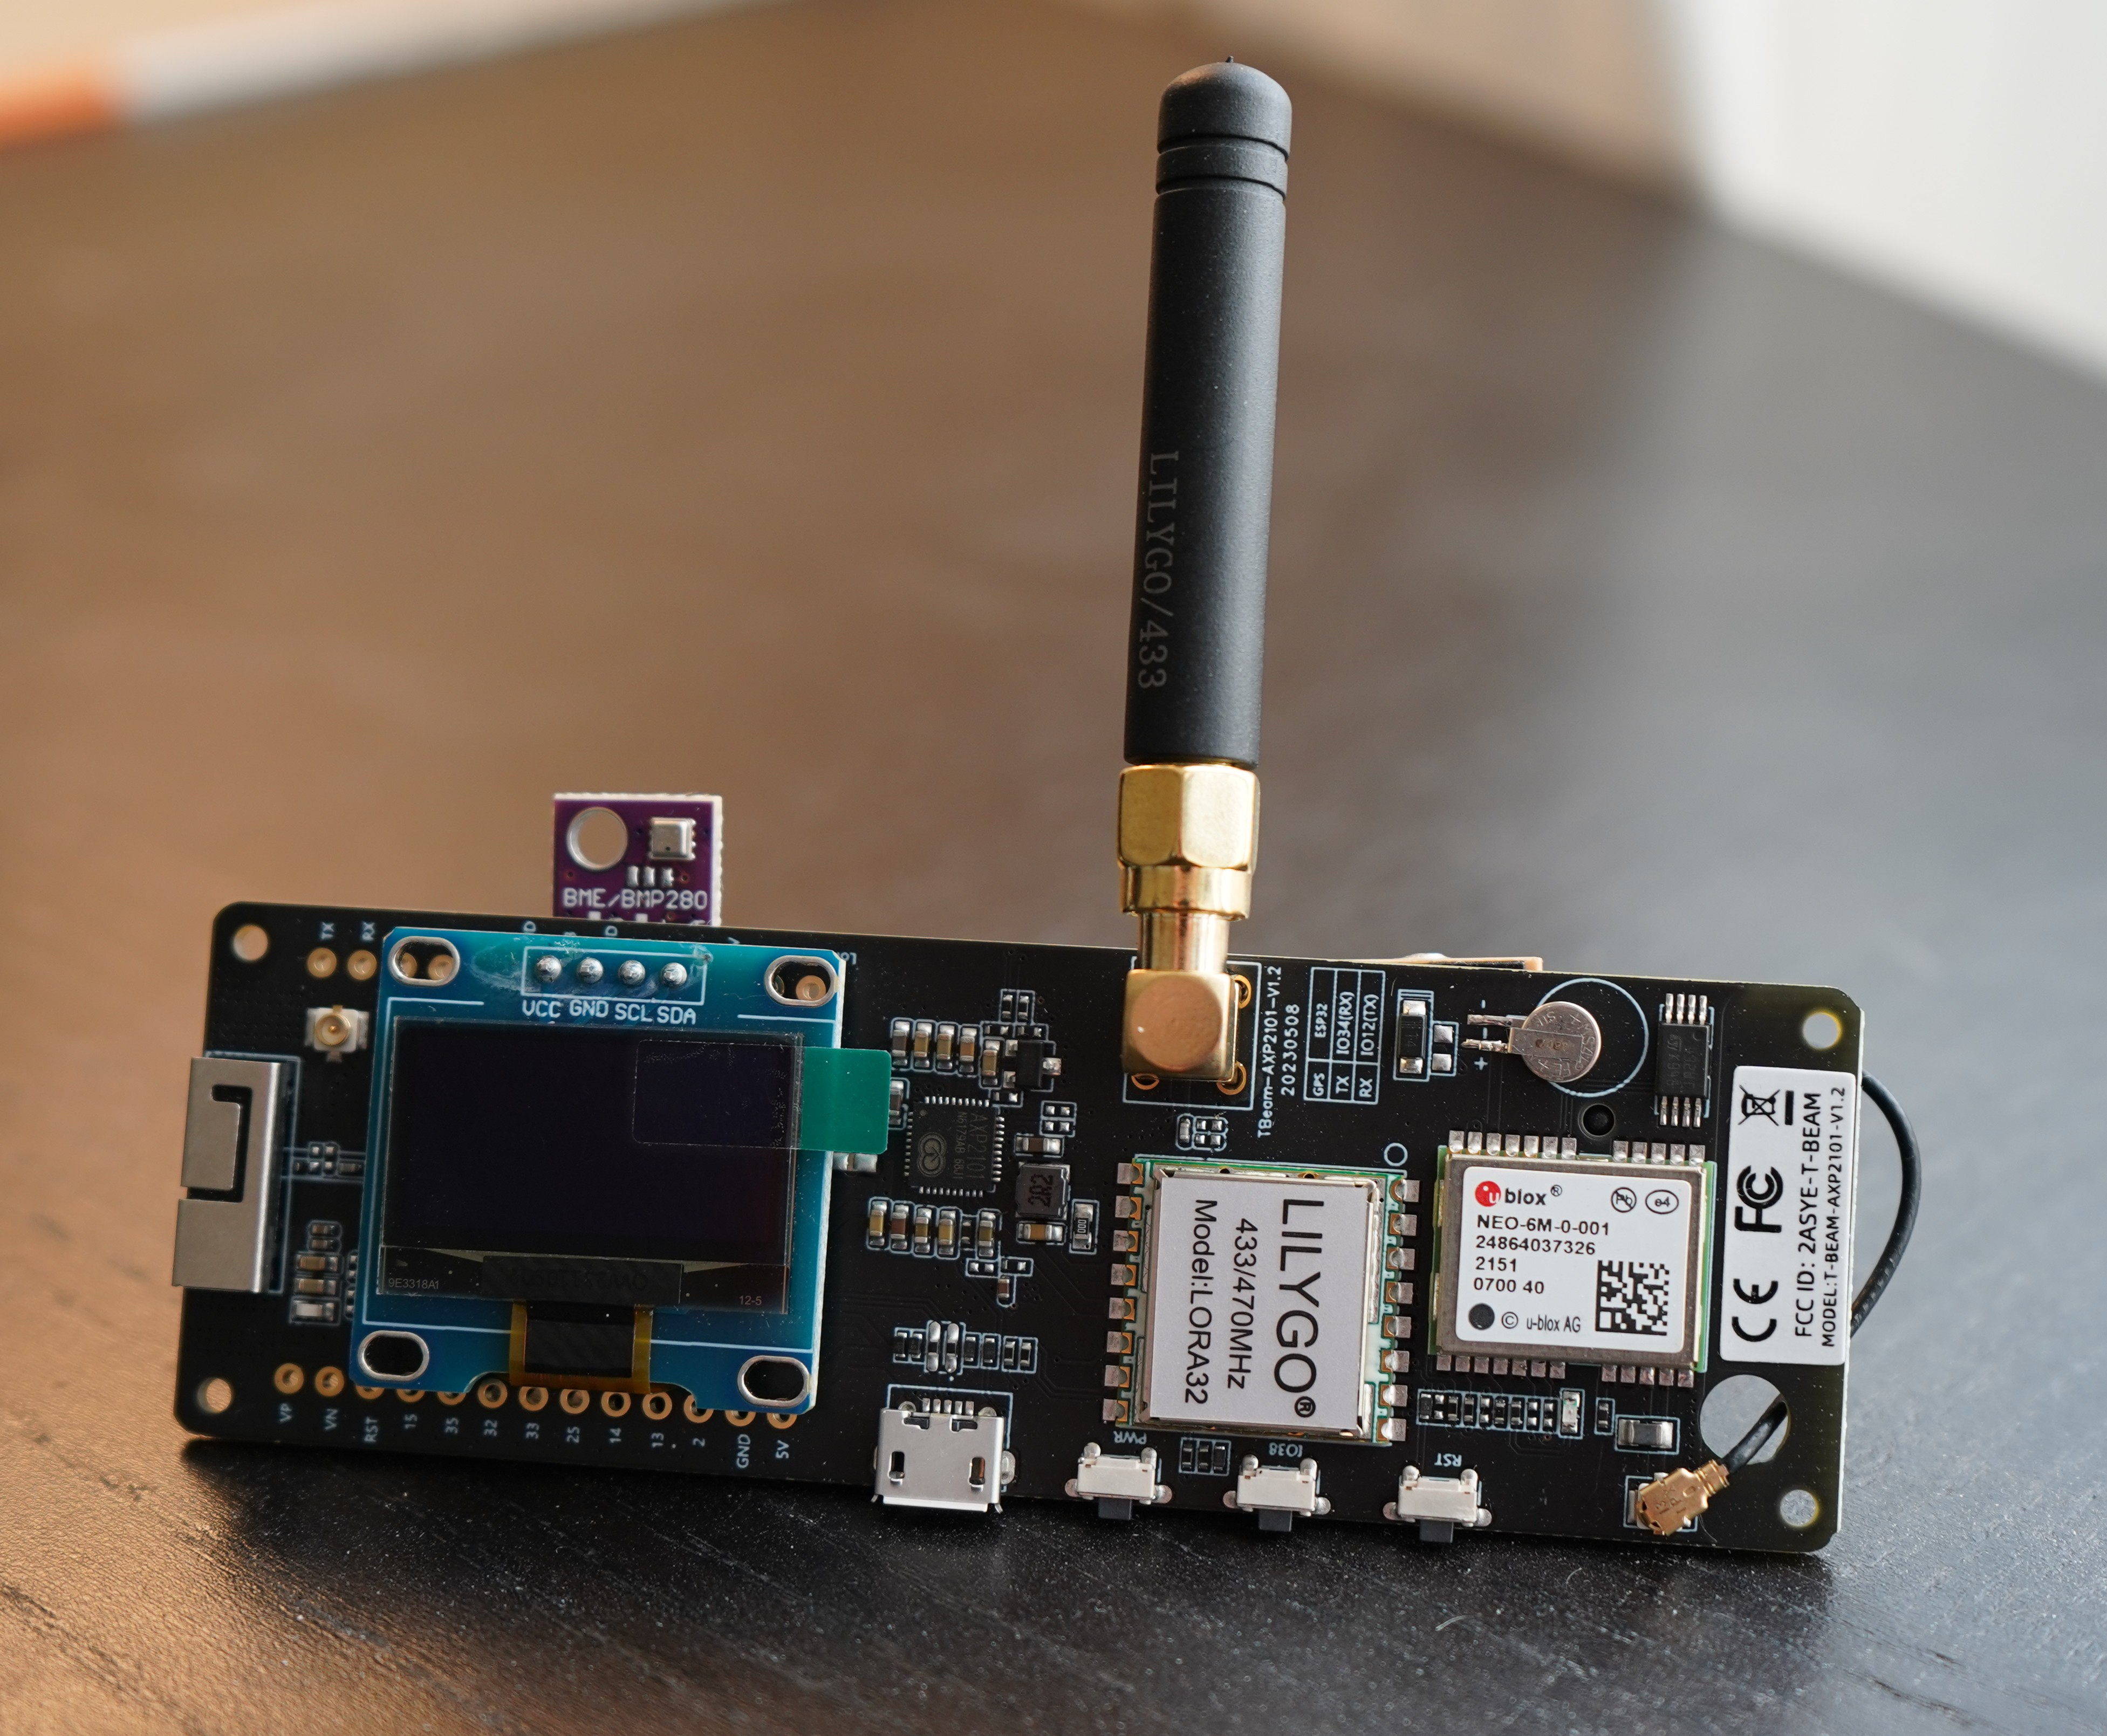
\includegraphics[height=6cm,keepaspectratio]{images/tbeam.jpg}
    \end{column}
  \end{columns}
\end{frame}

\begin{frame}[fragile]
  \frametitle{Modem Presets}
  Pre-defined settings which define bandwidth, spread factor, and coding rate, all of which influence message speed and range/distance.
  \vfill{}
  \begin{description}[labelwidth=2cm]%[<+->]
    \item[\texttt{SHORT FAST}]{Fastest, highest bandwidth, lowest airtime, shortest range}
    \item[\texttt{SHORT SLOW}]{}
    \item[\texttt{MEDIUM FAST}]{}
    \item[\texttt{MEDIUM SLOW}]{}
    \item[\texttt{LONG FAST}]{Default modem preset, best performance/range balance}
    \item[\texttt{LONG MODERATE}]{}
    \item[\texttt{LONG SLOW}]{}
    \item[\texttt{VERY LONG SLOW}]{Slowest, lowest bandwidth, highest airtime, longest range. Not recommended for anything other than range tests}
  \end{description}
\end{frame}

\section{Custom Sensors}
\frame{\sectionpage}
\begin{frame}[fragile]
  \frametitle{Meshtastic Telemetry}
  \begin{columns}[]
    \begin{column}[T]{0.45\paperwidth}
      \begin{itemize}%[<+->]
        \item{Easy to set up and use}
        \item{Allow for specific, inexpensive, widespread sensors}
        \item{Similar integrations with ESPHome (though not as extensive)}
     \end{itemize}
    \end{column}
    \begin{column}[T]{0.45\paperwidth}
      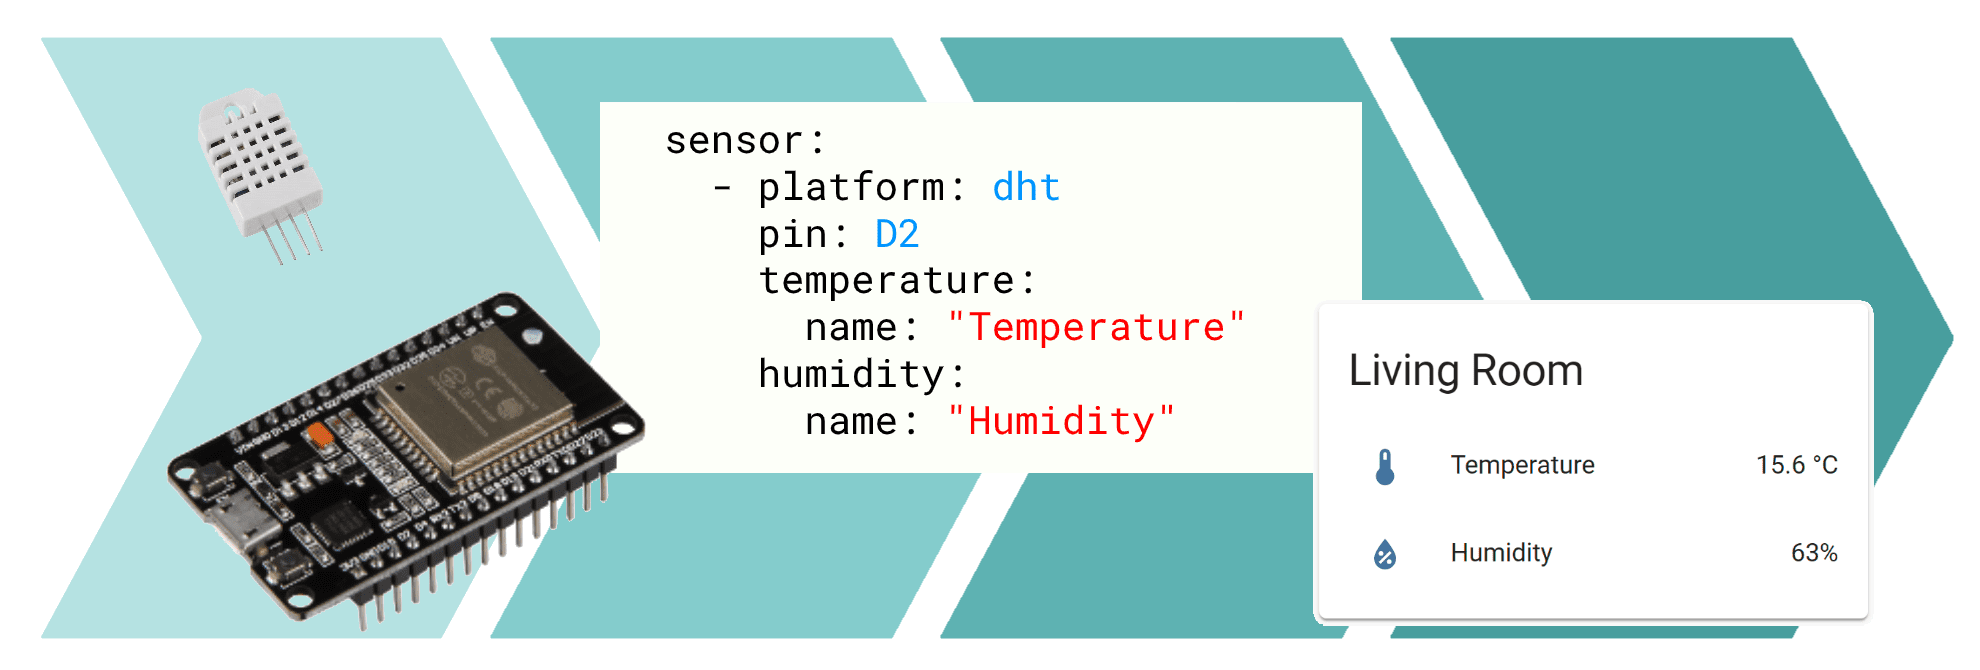
\includegraphics[width=0.45\paperwidth,keepaspectratio]{images/esp.png}
    \end{column}
  \end{columns}
\end{frame}

\subsection{Platforms}
% Devices/Components
\subsection{Devices/Components}
\begin{frame}[fragile]
  \frametitle{Building Sensor Devices: The Sensors}
  \begin{columns}[]
    \begin{column}[T]{0.45\paperwidth}
      Currently supported `sensor components':
      \begin{description}[leftmargin=2cm]%[<+->]
        \item[MCP9808]{Temperature}
        \item[BMP280]{Temperature, Barometric Pressure}
        \item[BME280]{Temperature, Barometric Pressure and Humidity}
        \item[BME680]{Temperature, Barometric Pressure, Humidity, Air Resistance}
        \item[INA260/INA219]{Current and Voltage}
        \item[SHTC3/SHT31]{Temperature and Humidity}
        \item[PMSA003I]{Air Quality Index/VOC count}
      \end{description}
    \end{column}
    \begin{column}[T]{0.45\paperwidth}
      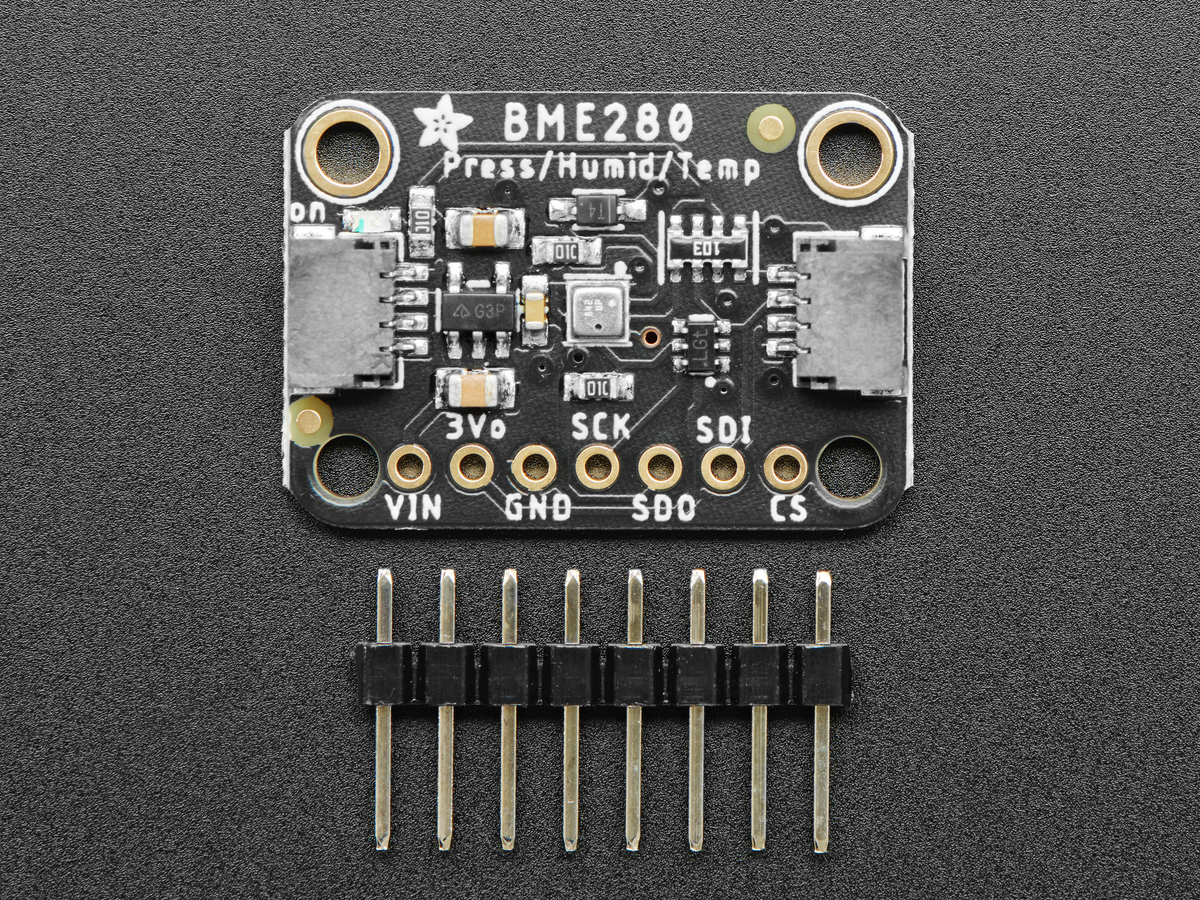
\includegraphics[width=0.45\paperwidth,keepaspectratio]{images/bme280-ada.jpg}
    \end{column}
  \end{columns}
\end{frame}

% Platforms
\begin{frame}[fragile]
  \frametitle{Building Sensor Devices: Hooking It Up}
  \begin{columns}[]
    \begin{column}[T]{0.45\paperwidth}
      \begin{itemize}
        \item{Meshtastic has built-in support for a number of devices via I$^2$C.}
        \item{Typical cost for a sensor module can be as low as \$1}
        \item{Sensors are usually simply wired up to the I$^2$C ports, but specific device models vary.}
        \item{\color{red}{BME280 Sensor for Temperature, Humidity, Air Pressure}}
        %\item{\color{cyan}{UBlox GPS Sensor for location, time, and altitude}}
      \end{itemize}
    \end{column}
    \begin{column}[T]{0.45\paperwidth}
      % Annotate on picture from
      % https://tex.stackexchange.com/questions/9559/drawing-on-an-image-with-tikz#9561
      \begin{tikzpicture}
        \node[anchor=south west,inner sep=0] (image) at (0,0) {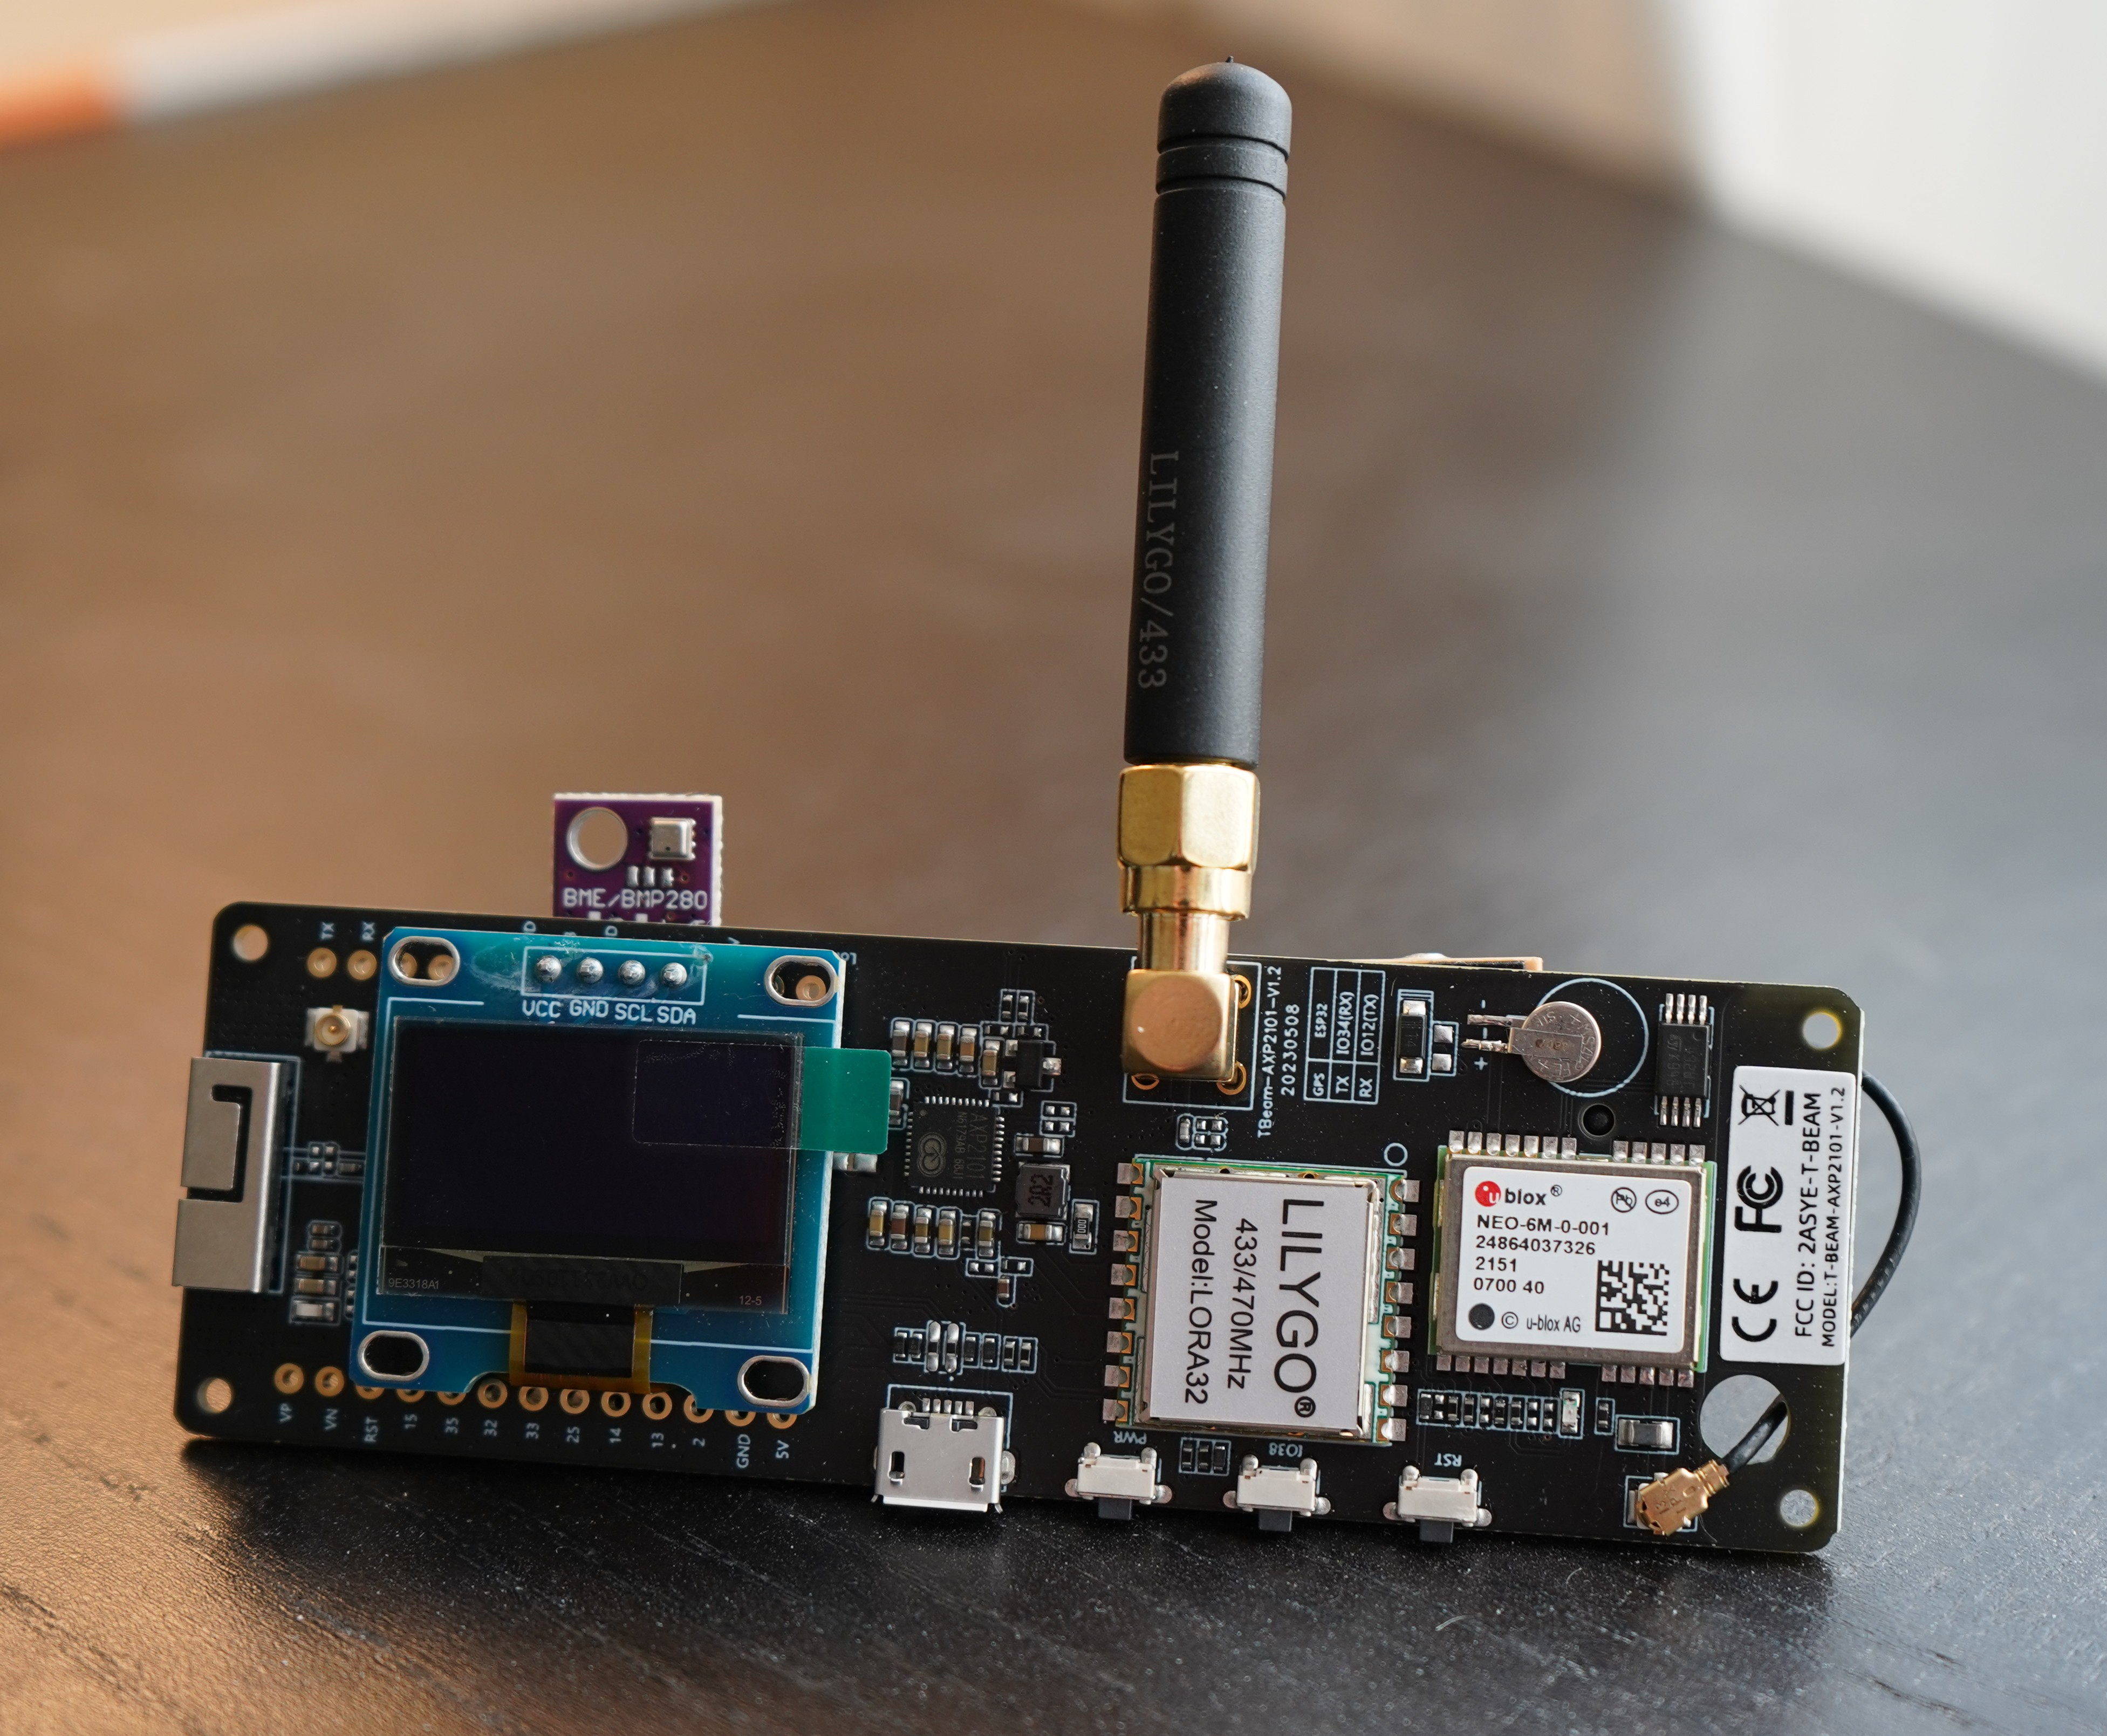
\includegraphics[height=6cm]{images/tbeam.jpg}};
        \begin{scope}[x={(image.south east)},y={(image.north west)}]
          % Guide-lines
          %\draw[help lines,xstep=.1,ystep=.1] (0,0) grid (1,1);
          %\foreach \x in {0,1,...,9} { \node [anchor=north] at (\x/10,0) {0.\x}; }
          %\foreach \y in {0,1,...,9} { \node [anchor=east] at (0,\y/10) {0.\y}; }
          \draw[red,ultra thick,rounded corners] (0.24,0.57) rectangle (0.36,0.42);
          %\draw[cyan,ultra thick,rounded corners] (0.66,0.37) rectangle (0.82,0.19);
        \end{scope}
      \end{tikzpicture}
    \end{column}
  \end{columns}
\end{frame}

\section{Usage and Demo}
\subsection{Demo of Meshtastic}
\frame{\subsectionpage}

\subsection{Looking at the Meshtastic Signal}
\frame{\subsectionpage}

\section{Wrapping Up}
\frame{\sectionpage}

\begin{frame}
  \frametitle{Key Takeaways}
  \begin{itemize}[<+->]
    \item{Meshtastic is a great entry in to long range text communication}
    \item{There are a massive variety of tools and use cases for Meshtastic}
    \item{Useful for infrastructure-less, `off-grid' remote sensors}
    \item{Excellent way to ensure communication can `just work' in the event of an emergency}
  \end{itemize}
\end{frame}

\begin{frame}
  \frametitle{Thank You}
  \begin{center}
    \LARGE{Questions?}
    \vfill{}
    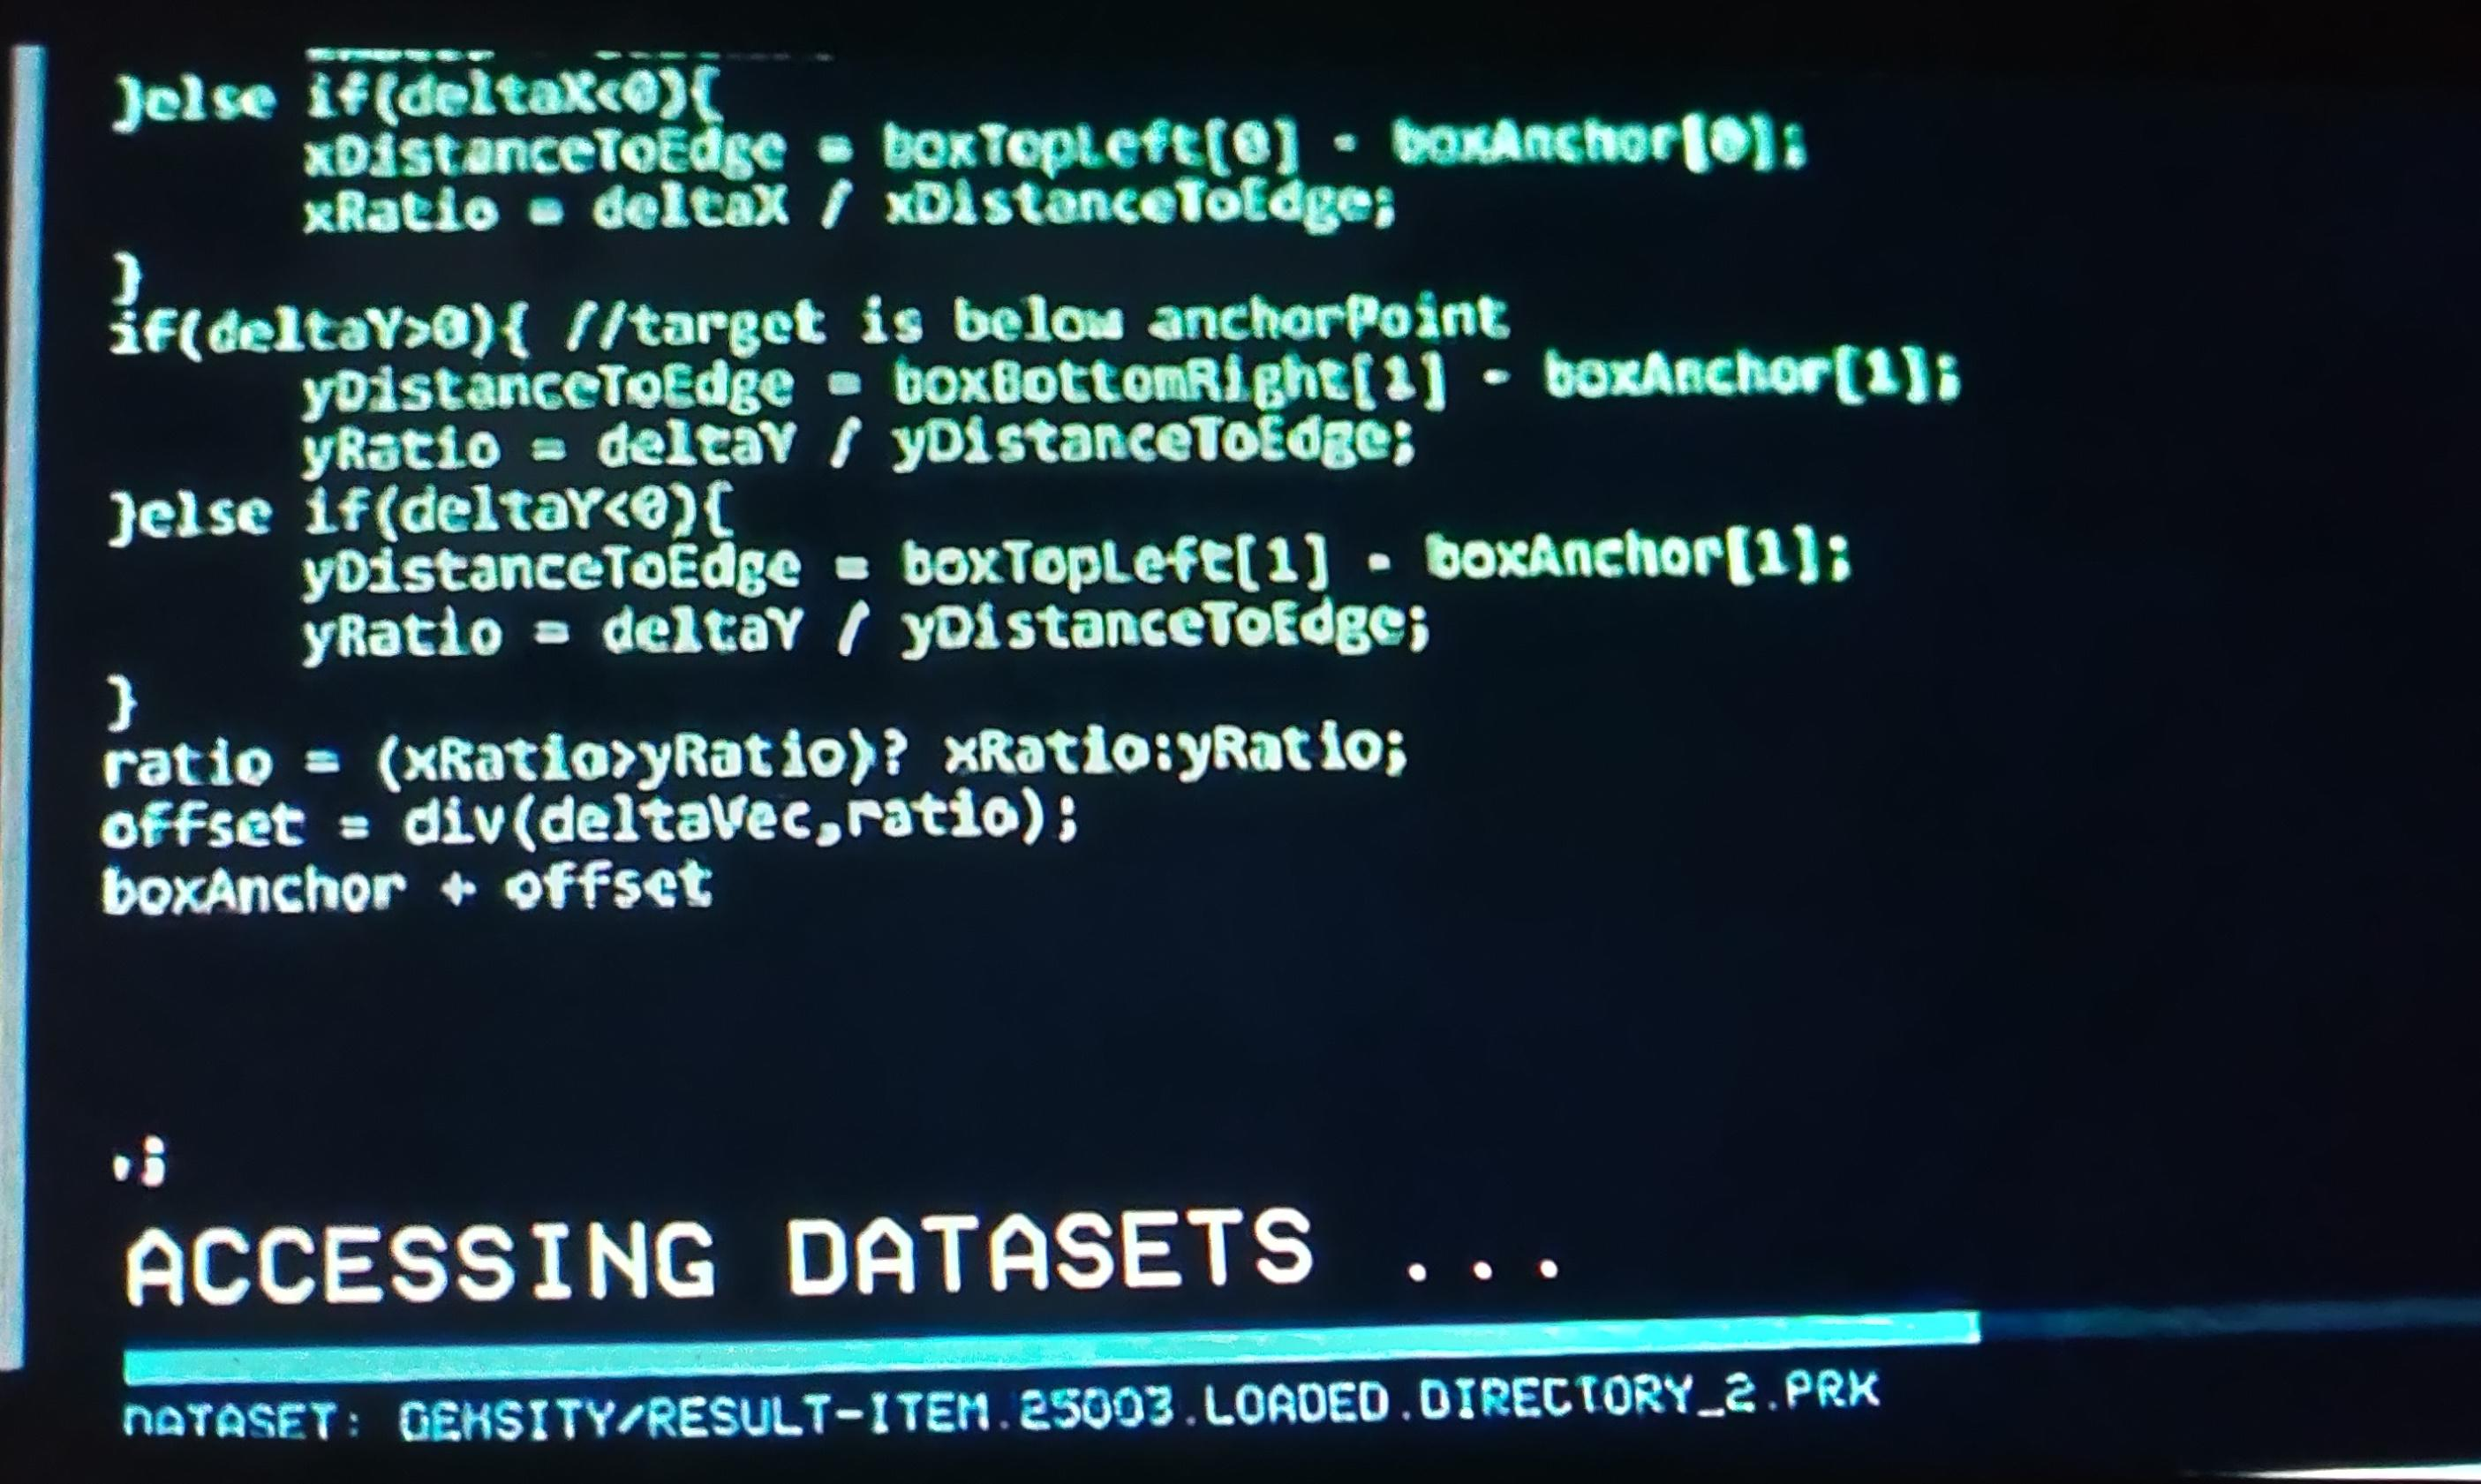
\includegraphics[height=5cm]{images/lol-code.jpg}
  \end{center}
\end{frame}
\begin{frame}[plain,fragile]
  \frametitle{References}
  \begin{columns}[]
    \begin{column}[T]{0.55\paperwidth}
      Code for this presentation, as well as some sample device manifests and other
      information can be found on GitHub and GitLab.
      \begin{itemize}
        \item{\href{https://github.com/tomswartz07/CPOSC2024}{https://github.com/tomswartz07/CPOSC2024}}
        \item{\href{https://gitlab.com/tom.swartz07/CPOSC2024}{https://gitlab.com/tom.swartz07/CPOSC2024}}
      \end{itemize}
      \vfill{}
      Further Reading:
      \begin{enumerate}
        \item{\href{https://meshtastic.org/}{https://meshtastic.org/}}
        \item{\href{https://hackaday.com/2023/06/26/meshtastic-for-the-greater-good/}{https://hackaday.com/2023/06/26/meshtastic-for-the-greater-good/}}
        \item{\href{https://store.rokland.com/pages/meshtastic-hardware-rak-lilygo}{https://store.rokland.com/pages/meshtastic-hardware-rak-lilygo}}
      \end{enumerate}
      \tiny{Legal Mumbo-jumbo:}
      \vfill{}
      \begin{itemize}
        \item{\tiny{Meshtastic\textsuperscript{\textsf{®}} is a registered trademark of Meshtastic LLC}}
      \end{itemize}
    \end{column}
    \begin{column}[T]{0.35\paperwidth}
      \qrcode[height=1.5in]{https://github.com/tom.swartz07/CPOSC2024/}
    \end{column}
  \end{columns}
\end{frame}

\end{document}
% vim: set ts=2 sw=2 spell:
